\documentclass[10pt,twocolumn,letterpaper]{article}

\usepackage{cvpr}
\usepackage{times}
\usepackage{epsfig}
\usepackage{graphicx}
\usepackage{amsmath}
\usepackage{amssymb}

% Include other packages here, before hyperref.
\usepackage{subcaption}

% If you comment hyperref and then uncomment it, you should delete
% egpaper.aux before re-running latex.  (Or just hit 'q' on the first latex
% run, let it finish, and you should be clear).
\usepackage[breaklinks=true,bookmarks=false]{hyperref}
\usepackage[capitalise, noabbrev]{cleveref}

\cvprfinalcopy % *** Uncomment this line for the final submission

% \def\cvprPaperID{****} % *** Enter the CVPR Paper ID here
\def\httilde{\mbox{\tt\raisebox{-.5ex}{\symbol{126}}}}

% Pages are numbered in submission mode, and unnumbered in camera-ready
\ifcvprfinal\pagestyle{empty}\fi
% \setcounter{page}{4321}
\begin{document}

%%%%%%%%% TITLE
\title{COMP6223 Coursework 2: Subverting Face Detection}

\author{Eugene Teoh\\
Electronics and Computer Science, University of Southampton\\
Southampton, UK\\
{\tt\small wct1c16@soton.ac.uk}
}

\maketitle
%\thispagestyle{empty}

%%%%%%%%% ABSTRACT
% \begin{abstract}

% TODO: Talk about why subverting face detectors are a big deal. Real life applications etc.
   
% \end{abstract}

%%%%%%%%% BODY TEXT
\section{Introduction}

% TODO: Introducing what this coursework is about

This report presents the results and findings for the tasks stated in COMP6223 coursework 2. In this report, different types of camouflages are explored and added to my own face in hopes of subverting the Viola-Jones face detector \cite{viola-jones}. The only condition imposed in the coursework is that the camouflage should be non-invasive and have minimal occlusion.

\section{Viola-Jones Object Detector}

Viola-Jones, or Haar Cascade face detector was proposed by Viola and Jones~\cite{viola-jones} in 2001. The framework uses three main concepts, namely: ``Integral Image'', AdaBoost feature selection and cascade classifier.

First, a subwindow (originally 24 $\times$ 24) is chosen. Within the subwindow, the author proposed the use of four Haar-like features to match every pixel. In a 24 $\times$ 24 subwindow, there exist a set of over 160,000 features. The subwindow is shifted over the the image, similar to a convolution operation.

Integral Image was proposed to be able to calculate the sum of values of a block of pixels in linear time, more specifically in just 4 steps. This will significantly improve the speed of calculation of the 160,000 Haar-like features.

Next, AdaBoost, a boosting algorithm which transforms a set of weak classifiers into a strong classifier, is then used to select a smaller set of features with the largest weights.

Finally, the features selected is then ordered in a cascade of classifiers, more specifically a degenerate decision tree. For every subwindow, if the values of the features passes through every classifier of the cascade, a face is detected.


\section{Camouflages}

% TODO: Prominent Features

Subversion of the Viola-Jones face detector can be done by camouflaging face components. There are two main types of camouflage: concealment and deception \cite{facilitating-fashion-camouflage-art}. Both types of camouflage can be performed by occlusion, face paints, accessories (hat, glasses), jewellery and more.

Human faces consist of five major face components: face shape, eyes, eyebrows, nose and lip. All the face components stated above can be camouflaged with different tools. The sections below explore the effective camouflages for different face components. Other miscellaneous approaches for effective camouflages will also be explored in \cref{sec:miscellaneous}. It should be noted that camouflages for the lips were not found, thus will not be discussed in this section.

Almost all camouflages in this report are added to images of my face using GNU Image Manipulation Program (GIMP)~\cite{gimp}. This is due to the lack of accessories and tools to complete real, physical camouflages.

% It is often effective to camouflage prominent features. Feng and Prabhakaran~\cite{facilitating-fashion-camouflage-art} proposed a method to measure the statistical range of face components to identify prominent features using Active Appearance Models (AAM). We will not be exploring AAM as it is beyond the scope of this coursework. 

\subsection{Face Shape} \label{sec:face-shape}

\cref{fig:face-shape} shows an example of camouflage which attempts to modify the shape of the face. The camouflage used includes a face mask to deceive the chin area, a wig do alter the overall face structure, and a turban to change the forehead shape. The goal of the camouflage introduced is to modify the face shape into a non-round shape by introducing edges and curved surfaces.

Through empirical findings, it was difficult to find camouflages that was able to deceive the face detector with face shapes. The Viola-Jones algorithm might not have many features that emphasises on the face shapes.


\begin{figure}[t]
    \centering
    \begin{subfigure}[b]{.49\linewidth}
        \centering
        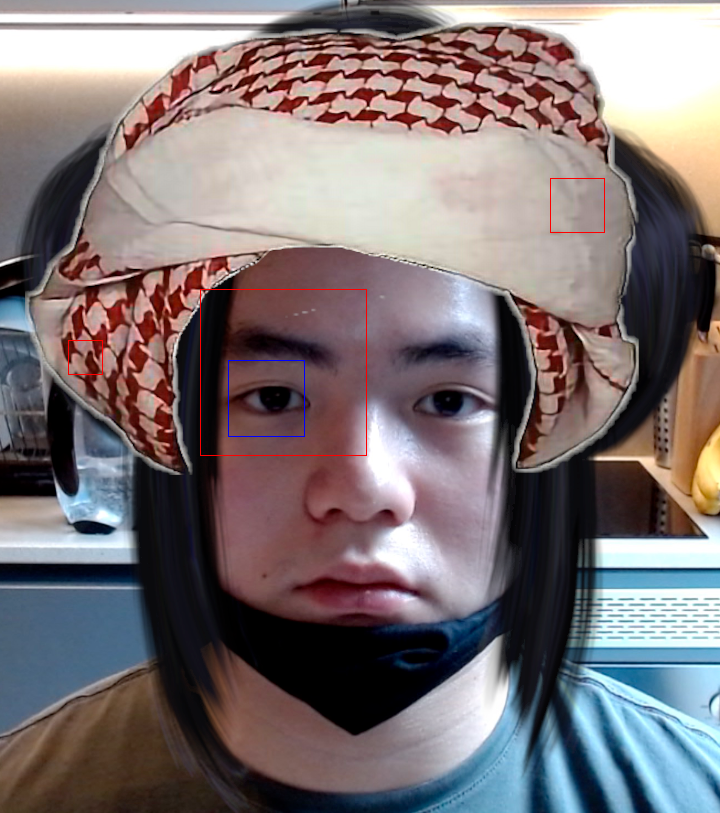
\includegraphics[width=\linewidth]{Figures/face_shape_1.png}
        \caption{Neutral}
    \end{subfigure}
    % \begin{subfigure}[b]{.49\linewidth}
    %     \centering
    %     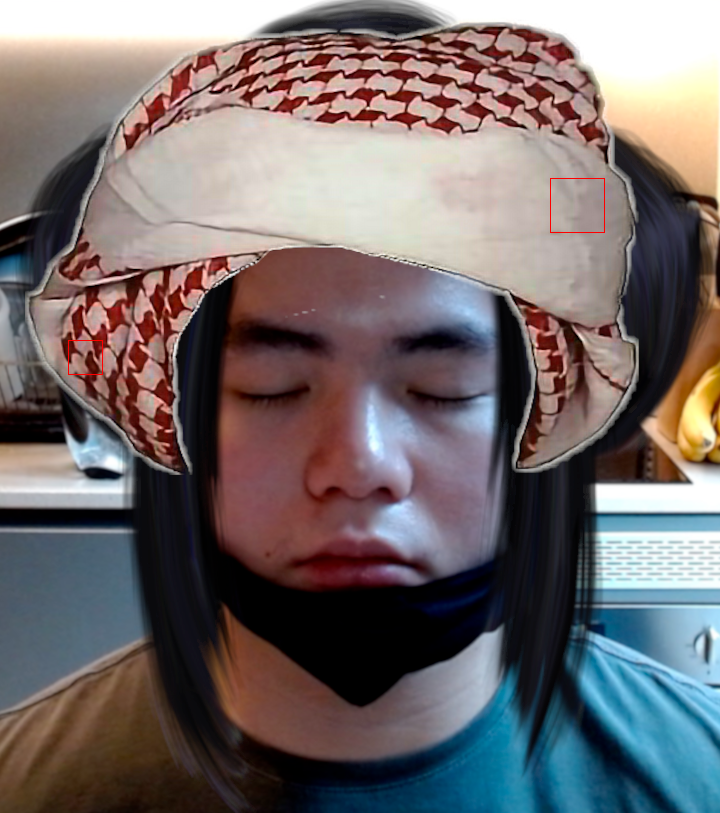
\includegraphics[width=\linewidth]{Figures/face_shape_2.png}
    %     \caption{Closed eyes}
    % \end{subfigure}
    \hfill
    \begin{subfigure}[b]{.49\linewidth}
        \centering
        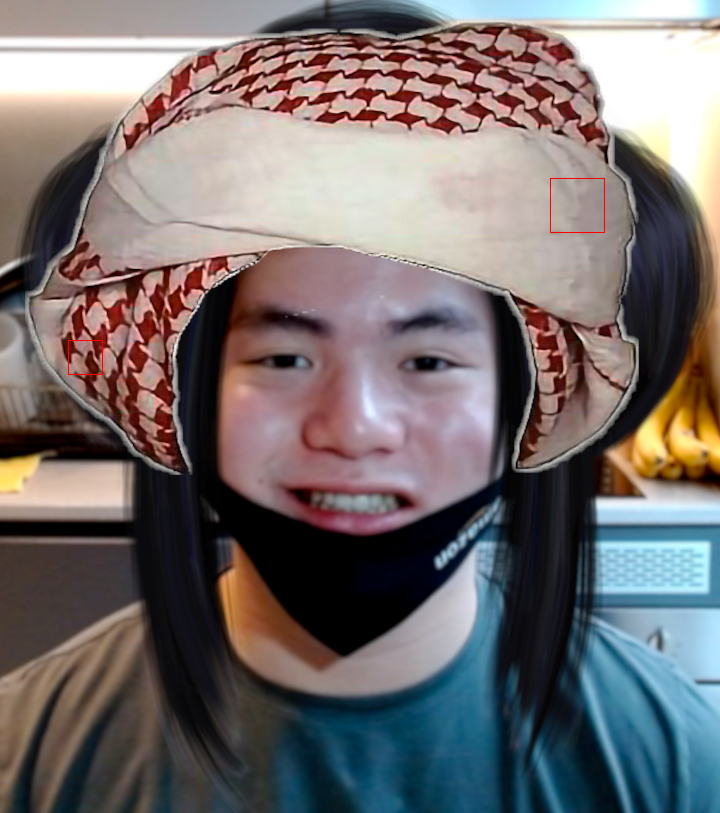
\includegraphics[width=\linewidth]{Figures/face_shape_3.png}
        \caption{Smiling}
    \end{subfigure}
    
    
    \caption{Face shape camouflage using face covering, wig (Sourced from \cite{wig}) and turban (Sourced from \cite{turban}) with face detection results of OpenCV online face detection tool.}
    \label{fig:face-shape}
\end{figure}

\subsection{Eyes and Eyebrows} \label{sec:eyes}

\cref{fig:eyes} shows an example of camouflage which attempts to occlude eyebrows and facial features around the eyes. The camouflage used is a domino mask used by DC Comic's fictional character, Robin.

From personal observations and other empirical findings~\cite{cvdazzle}, it is identified that the area that intersects both eyes, and the area between the eyebrows and eyes are important features for the face detector. This is possibly due to the obvious significant difference of pixel values between those areas. By adding a black domino mask as a camouflage, there will be less difference in pixel values between those areas. Hence, it causes the Haar-like features (especially the black-white-black features) to have values indifferent to the classifier thresholds.

In addition, equipping myself with a Robin domino mask gives me the ability to be Batman's side-kick and fight crimes in the dark, hence being undetectable from face detectors.

\begin{figure}[t]
    \centering
    \begin{subfigure}[b]{.49\linewidth}
        \centering
        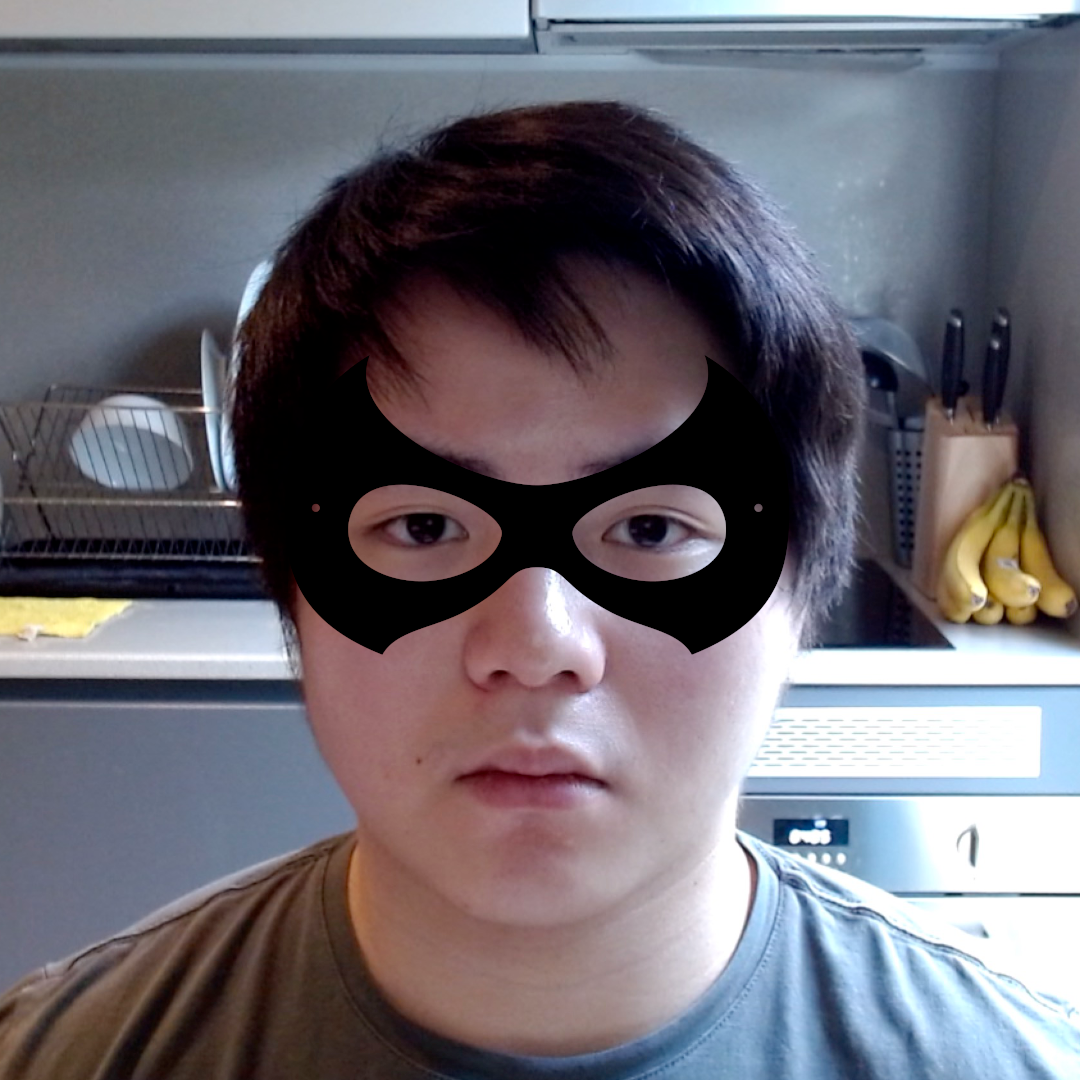
\includegraphics[width=\linewidth]{Figures/eyes_1.png}
        \caption{Neutral}
    \end{subfigure}
    % \begin{subfigure}[b]{.49\linewidth}
        % \centering
        % 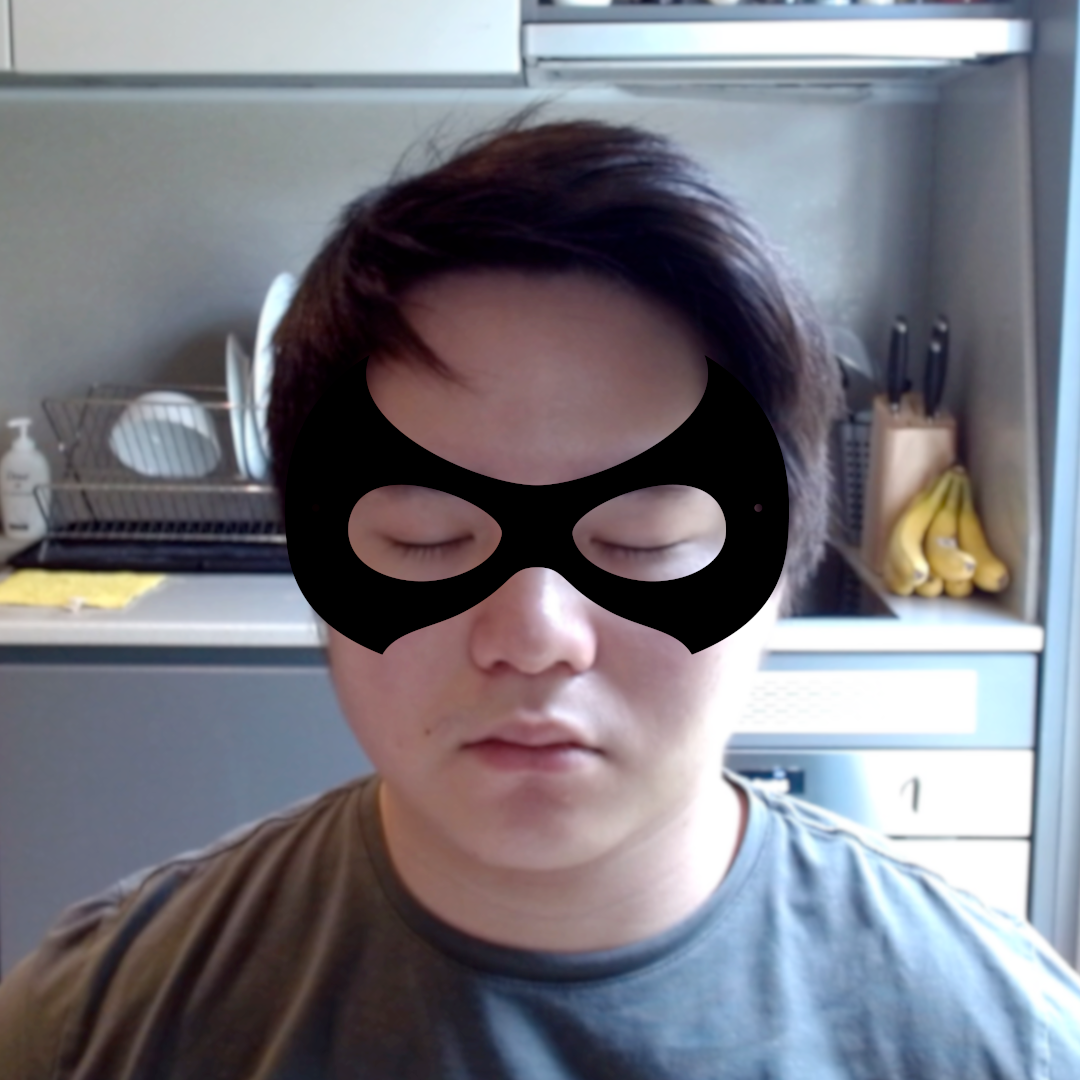
\includegraphics[width=\linewidth]{Figures/eyes_2.png}
        % \caption{Closed eyes}
    % \end{subfigure}
    \hfill
    \begin{subfigure}[b]{.49\linewidth}
        \centering
        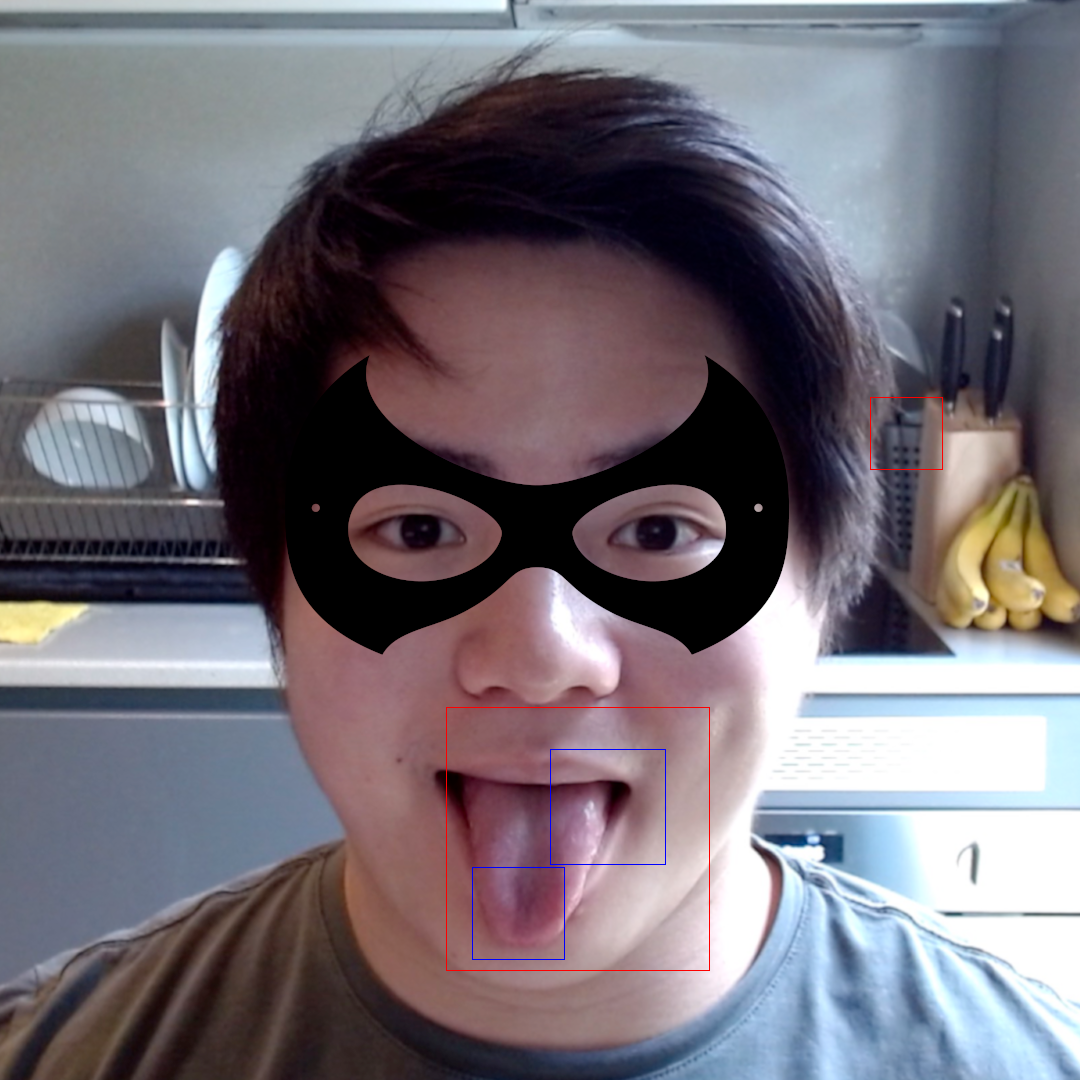
\includegraphics[width=\linewidth]{Figures/eyes_3.png}
        \caption{Smiling with tongue out}
    \end{subfigure}
    
    \caption{Eyes camouflage using Robin mask (Sourced from \cite{robin}) with face detection results of OpenCV online face detection tool.}
    \label{fig:eyes}
\end{figure}


\subsection{Nose}

\cref{fig:nose} shows an example of camouflage on the nose bridge area. Using the paint brush function in GIMP, a grey colour was used to paint the nose bridge area. Gaussian blur is then applied to the paint repeatedly until it is observationally realistic. This approach is synonymous to when real face paint is applied to face.

With minimal effort, by just painting the nose bridge area, subversion of the face detector is achieved. Similar to \cref{sec:eyes}, the Viola-Jones algorithm also prioritise on features around the nose bridge area. This is due to the significant difference of pixel values in that particular area. By applying ``artificial'' face paint, the Haar-like features will produce an output very indifferent of the threshold for the classification.

\begin{figure}[t]
    \centering
    \begin{subfigure}[b]{.49\linewidth}
        \centering
        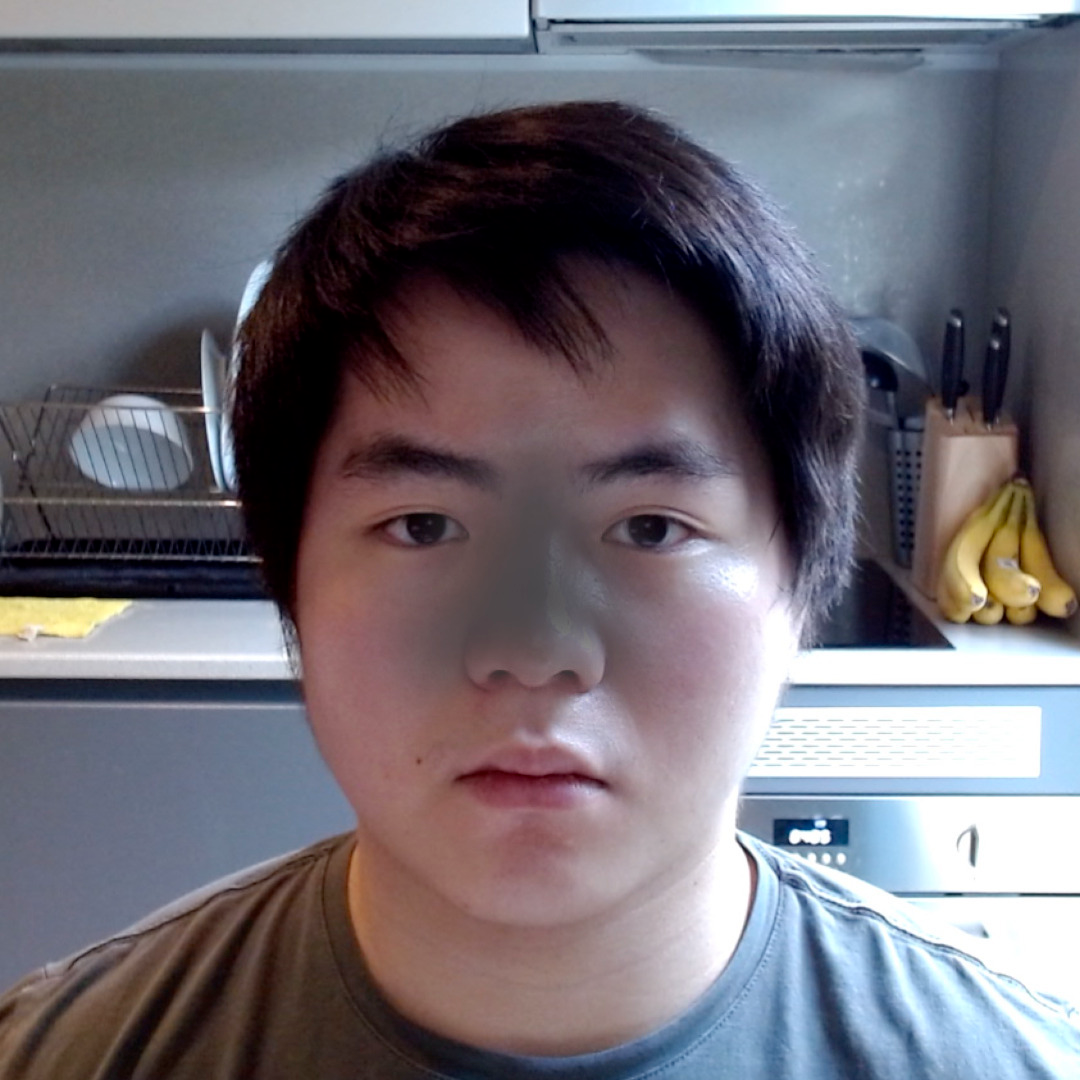
\includegraphics[width=\linewidth]{Figures/nose_1.png}
        \caption{Neutral}
    \end{subfigure}
    % \begin{subfigure}[b]{.49\linewidth}
    %     \centering
    %     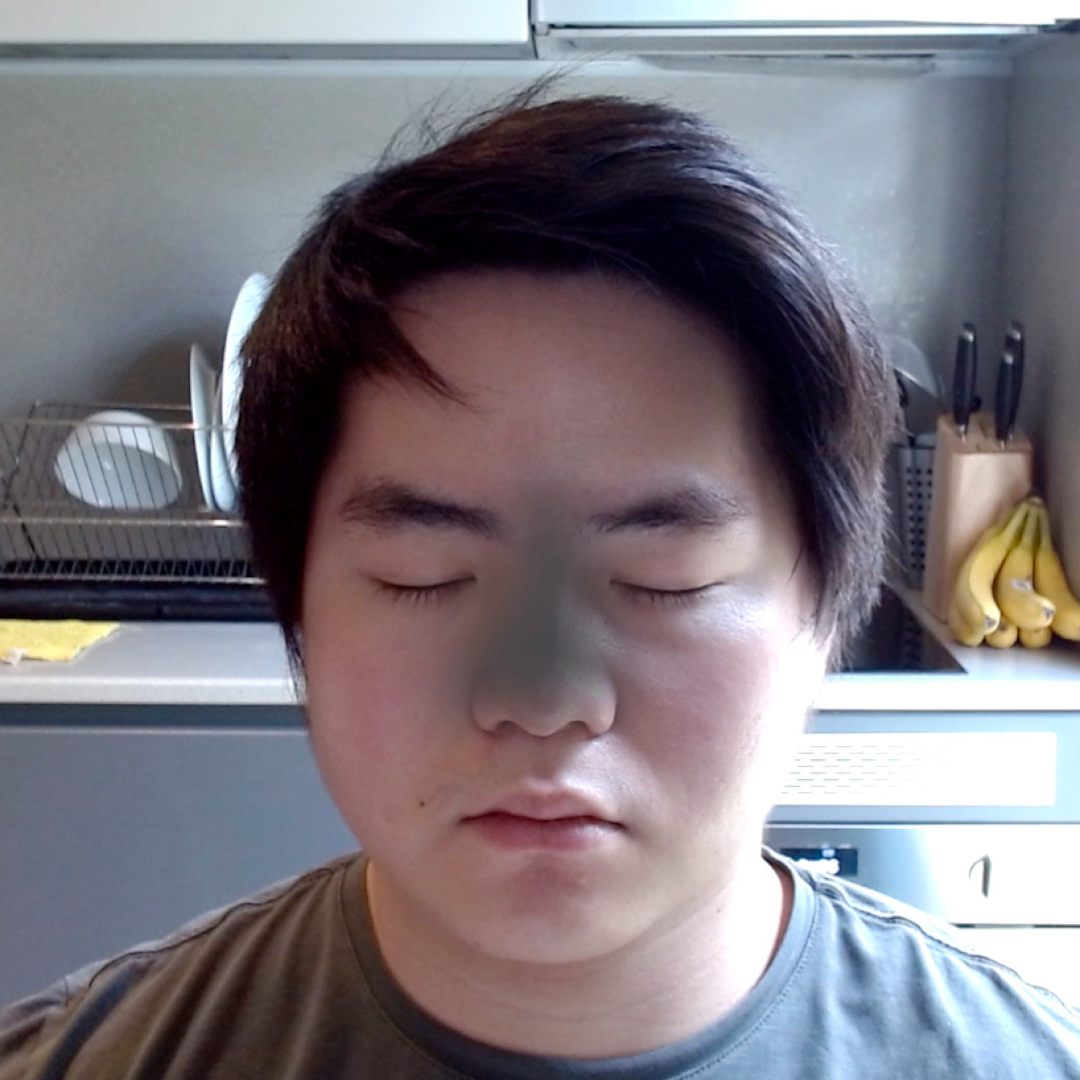
\includegraphics[width=\linewidth]{Figures/nose_2.png}
    %     % \caption{Closed eyes}
    % \end{subfigure}
    \hfill
    \begin{subfigure}[b]{.49\linewidth}
        \centering
        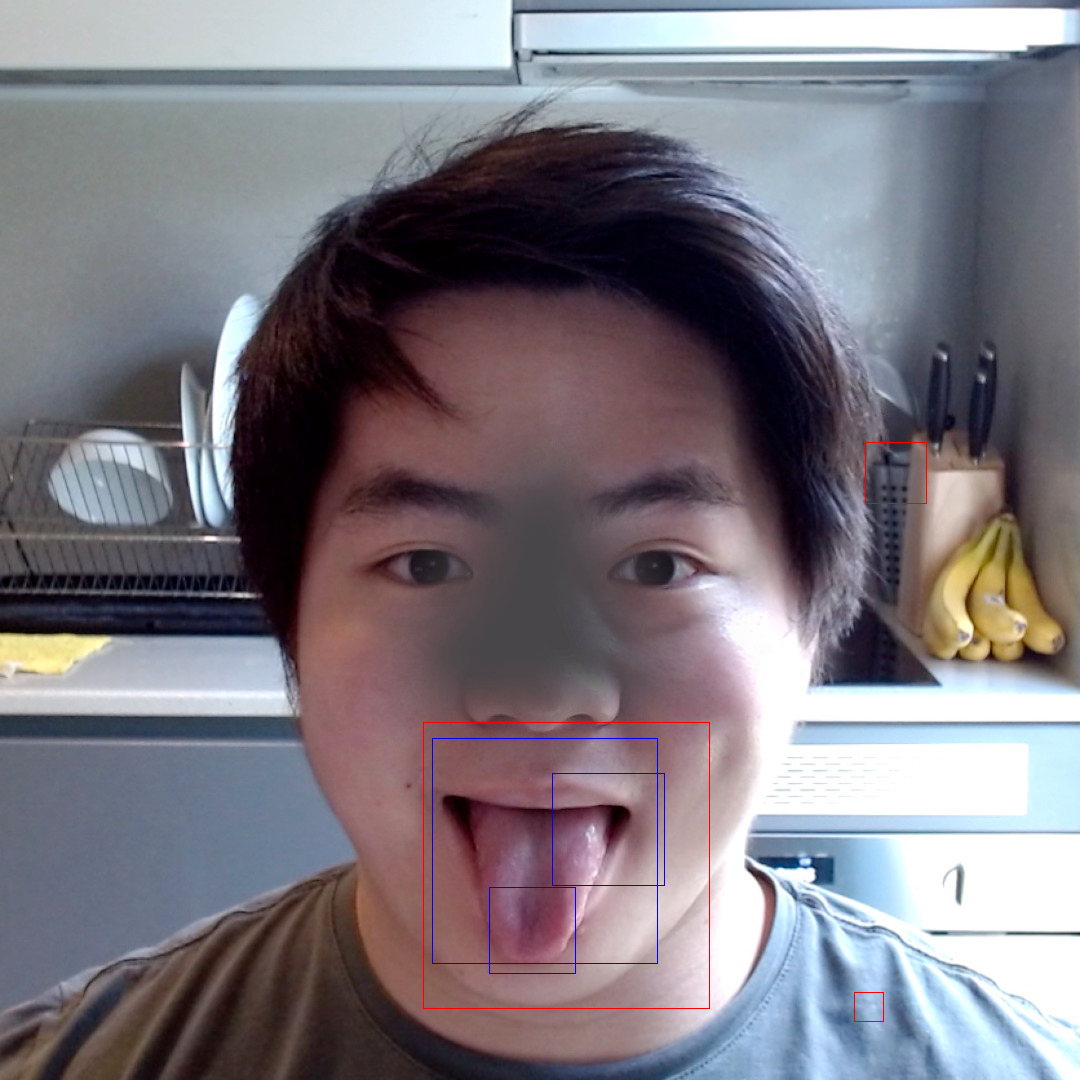
\includegraphics[width=\linewidth]{Figures/nose_3.png}
        \caption{Smiling with tongue out}
    \end{subfigure}
    
    \caption{Nose camouflage using face paint with face detection results of OpenCV online face detection tool.}
    \label{fig:nose}
\end{figure}


\subsection{Miscellaneous} \label{sec:miscellaneous}

There is a non-exhaustive list of approaches to subverting the face detector. There are two other approach that was found to be effective to the Viola-Jones algorithm.

First is to combine approaches from the previous sections to camouflage several face components at once. \cref{fig:thug-life} shows and example of camouflaging several face components.

Another approach that is found to be effective is asymmetry. Harvey~\cite{cvdazzle} identified that asymmetry between left and right side of the face will allow for more effective camouflage. \cref{fig:face-paint} shows an example of asymmetric face paint applied using GIMP's paint brush and gaussian blur.



\begin{figure}[t]
    \centering
    \begin{subfigure}[b]{.49\linewidth}
        \centering
        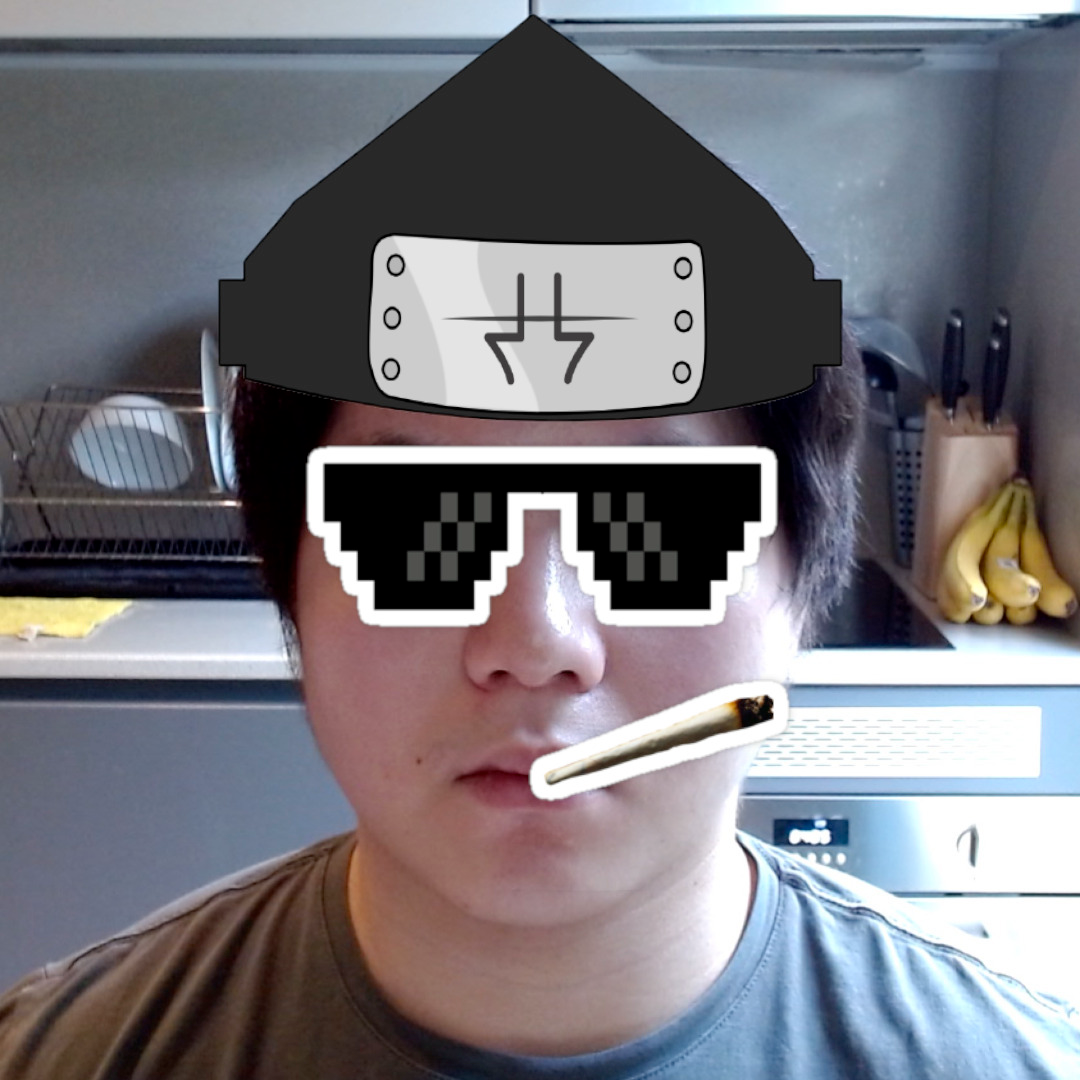
\includegraphics[width=\linewidth]{Figures/combined.png}
        \caption{Camouflage with ninja bandana and ``thug life'' meme glasses and cigarette}
        \label{fig:thug-life}
    \end{subfigure}
    % \begin{subfigure}[b]{.49\linewidth}
    %     \centering
    %     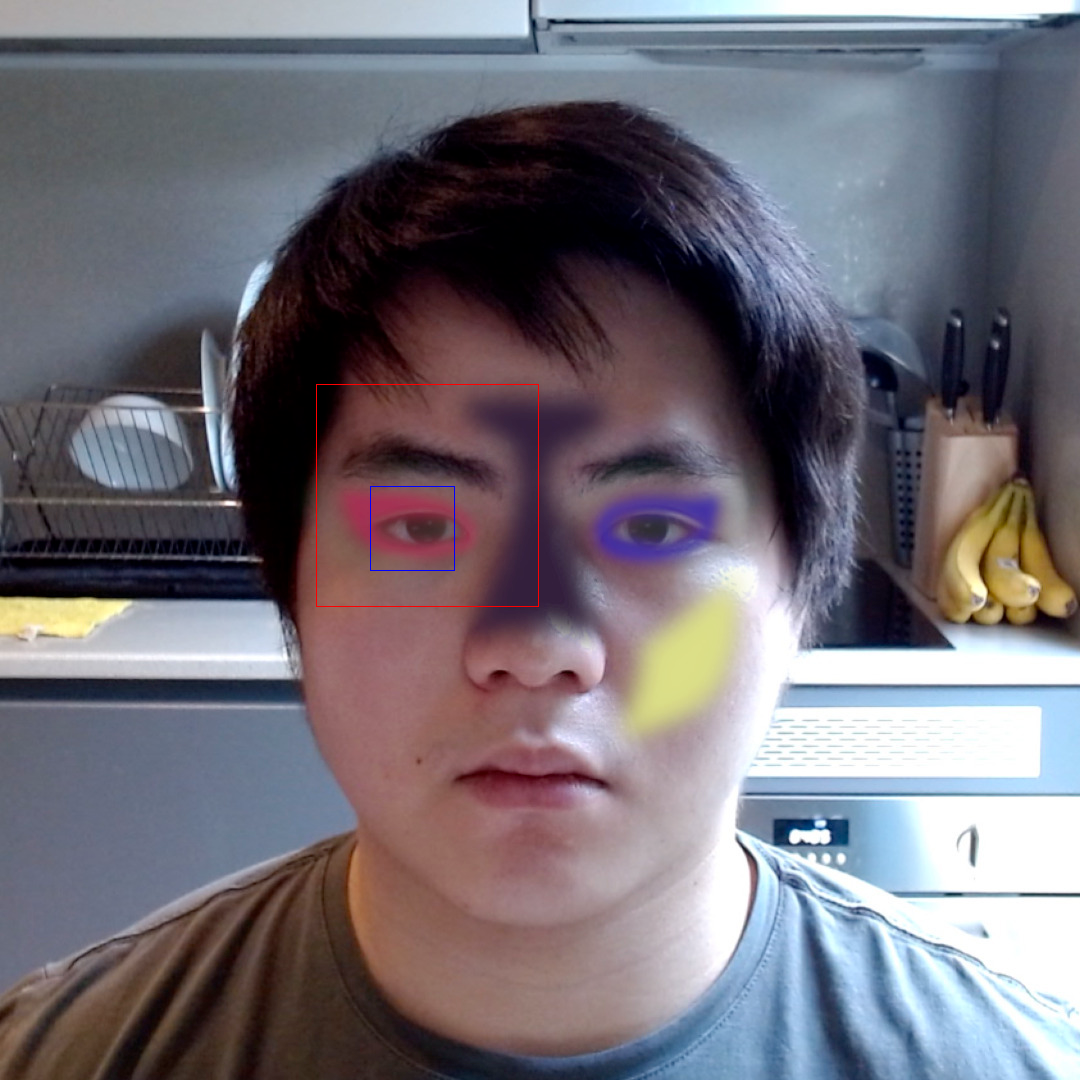
\includegraphics[width=\linewidth]{Figures/combined2.png}
    %     % \caption{Closed eyes}
    % \end{subfigure}
    \hfill
    \begin{subfigure}[b]{.49\linewidth}
        \centering
        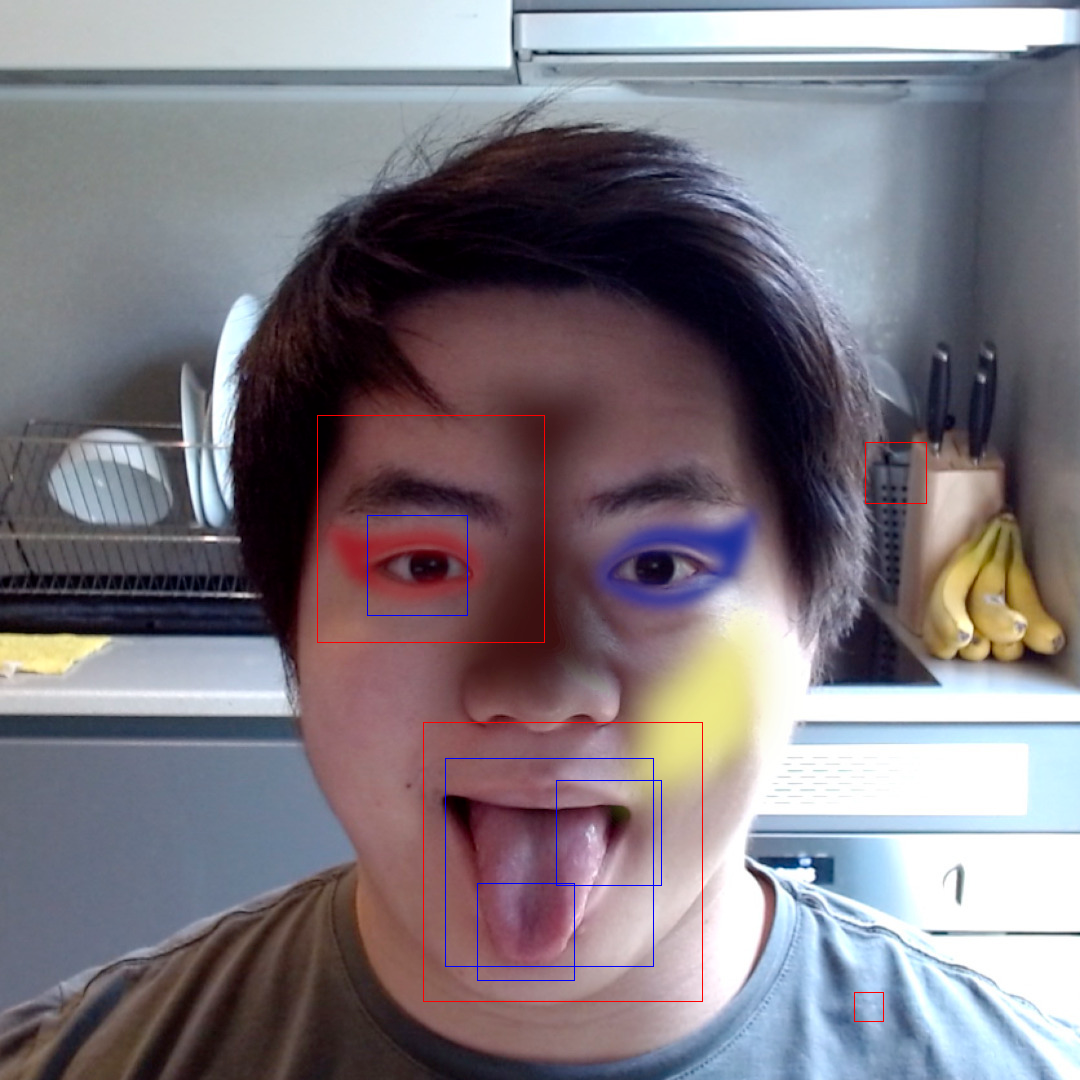
\includegraphics[width=\linewidth]{Figures/combined2_2.png}
        \caption{Camouflage with asymmetric colour and position of face paint}
        \label{fig:face-paint}
    \end{subfigure}
    
    \caption{Miscellaneous camouflages (Sourced from \cite{naruto,thug-life}) with face detection results of OpenCV online face detection tool.}
    \label{fig:others}
\end{figure}






% \section{Conclusion}

% Hello world!


\pagebreak

{\small
\bibliographystyle{ieee_fullname}
\bibliography{egbib}
}

\end{document}


